\chapter{General Considerations}
\label{cha:Lush_Chapter_39}
\index{Inbreeding|(}

In the preceding chapters each of the methods by which the breeder
can change the genetic composition of a breed has been examined to see
what it will and what it will not do and hence under what circumstances
it would be useful. Before passing to the individual breeder's plans
for his own procedure it is appropriate to review for a moment what
each of the tools available to him will do best.

\index{Selection}
Selection --- i.e., differences in the number of offspring which different
kinds of individuals are permitted to have --- is the most effective
method for changing the frequency of genes and the genetic averages of
the breed for various characteristics. It is naturally the method the
breeder considers first because his profit or loss will depend mostly upon
the average merit of the stock which he produces for sale. So far as genes
produce effects which are consistently desirable in all combinations
with other genes, the changes produced by selection are permanent
(unless and until equally effective counter-selection has taken place);
but insofar as the effects of the genes are desirable in some combinations
and undesirable in others, many of the changes which selection
produces when it is first practiced are lost within a generation or two if
selection ceases. Selection produces only slight changes in the homozygosity
or uniformity of a population unless it continues over many generations.
If there is much epistasis, selection may increase uniformity
rather sharply when first practiced; but continued selection is necessary
to hold that increase in uniformity. Selection does not change the uniformity
of the next generation nearly as much as it changes the average.
The usefulness of selection can almost be summarized by saying that it
usually carries the breeder toward his goal but is almost powerless to do
much toward ``fixing'' characteristics. In cases where there is much epistasis,
the rate of progress in changing the herd or breed average slackens
considerably after the first few generations.

Inbreeding is in many respects a perfect complement to selection; it
can do what selection cannot do, and can do feebly or not all that which
selection can do well. Inbreeding is uniquely powerful as a means of
producing homozygosity and prepotency or genuine ``fixity'' of type. It
produces uniformity within the various inbred lines but marked differences
between lines. Thus, it leads to the apparent paradox of a very
non-uniform breed composed of very uniform lines or families. Because
of its family-forming power, inbreeding can make selection much more
effective, especially in cases where there is much epistasis. Inbreeding
which is directed toward keeping relationship to some admired ancestor
high (i.e., linebreeding) is a combination of selection and inbreeding
particularly useful for perpetuating favorable epistatic effects of certain
gene combinations.

\index{Outbreeding}
Outbreeding promotes individual merit by tending to conceal recessive
genes. It remedies damage done by inbreeding and is useful for
introducing desirable genes into a population which lacks them.
Because it destroys family distinctness, covers recessives and scatters
favorable epistatic combinations, outbreeding hinders progress in breed
improvement except in those cases where a little outcrossing is necessary
to introduce desired genes into a family which lacks them. Outbreeding
is primarily a method for the producer of market animals.

The breeding of outwardly similar individuals together has practically
no effect upon homozygosis or prepotency but does increase
immediately the average resemblance between parent and offspring.
\index{Assortive mating}
That happens merely because the parents are chosen for their resemblance
to each other and each offspring has a chance to inherit from
both parents genes which will make it seem like them both. Mating like
to like increases the proportion of extreme individuals and decreases
the proportion of intermediates, thereby making the population more
variable provided no accompanying selection is practiced. The effects of
mating like to like\index{Mating like to like} are limited by the correlation between genotype and
phenotype and cannot be extreme unless that correlation is high.
Hence, in practice, assortive mating based on somatic resemblance and
unaccompanied by selection does little but increase the variability of
the population. Mating unlikes\index{Mating unlikes} together to correct defects, where both
are too extreme but in opposite directions, makes the population more
uniform and keeps it nearer to an intermediate type. The mating of somatic
unlikes has little effect on homozygosis. It is a very useful breeding
system wherever the goal is an intermediate, particularly in a species
where fertility is moderate and some of the extreme individuals must be
used for parents.
\index{Inbreeding|)}

\section*{PLANS FOR INDIVIDUAL BREEDERS}
\index{Breeding systems for varied purposes|(}

\noindent
\textsc{For All Kinds of Breeders:}
\begin{enumerate}
	\item Decide what kind or type of animal and what level of production
	would be ideal for the breeder's own individual circumstances and
	local conditions.
	\item Find what living animals most nearly have the genes needed to produce
	that ideal animal.
	\begin{enumerate}
		\item By judging and testing each animal.
		\item By paying some attention to the merit of recent ancestors and
		close collateral relatives.
		\item By studying the progeny of each animal.
	\end{enumerate}
	\item Obtain, as far as can be done at reasonable prices, those animals
	which come nearest to having the ideal genes and let each have offspring
	in numbers proportional to the closeness with which its heredity approaches
	the ideal.
\end{enumerate}

\begin{multicols}{2}
	\noindent \textsc{For Breeders of Purebreds:}
	\begin{enumerate}
		\setcounter{enumi}{3}
		\item Keep the future herd closely related to the best animals of the present and of the recent past, letting the relationship to poor or ordinary animals be diluted by the natural halving effect of the processes of inheritance.
		\item Outcross only when it is necessary to prevent some serious defect from being fixed on the whole flock or herd. The higher the average individual merit of the herd and the farther the	breeder has gone in his line-breeding program, the milder and more tentative such outcrosses should be.
	\end{enumerate}
	\columnbreak

	\noindent \textsc{For Breeders of Market Animals}
	\begin{enumerate}
		\setcounter{enumi}{3}
		\item Outbreed so far as that can be done without using animals of distinctly poorer heredity than would be available if related individuals were mated together. By using sires which are bred but unrelated to the females on which they are to be used, the maximum of heterosis and individual merit can be kept without losing as much in uniformity as if the sires were not closely bred themselves.
	\end{enumerate}
\end{multicols}

\index{Adaptation to local conditions|(}
The first step in any animal breeding program is to decide what is
ideal. Until a breeder knows what kind of animal he wants, he is
stopped in his tracks and can neither select the best nor discard the
worst. Somewhat indefinite words, such as best, worst, poorer, better,
more productive, meritorious, etc., have intentionally been used in this
book instead of more precise words in discussing selection and kindred
problems because the purpose was to discuss ways of attaining the goals
the breeder wants and not to enter into the subject of what ideal for
each kind of animal would be most profitable. Each breeder needs to
consider his own physical and biological resources, his own markets and
his own personal inclinations to decide what characteristics his ideal
animals should possess. Naturally a beginning breeder would defer
somewhat to the opinions of those who have had more experience
under somewhat similar conditions, but his own conditions may be different
from those of the men from whom he is receiving advice. It seems
likely that the matter of local adaptability will receive more attention
in the future than it has in the past. Probably there will always be at
least enough interchange of breeding stock to keep that from being
overdone. The ideal must often be a compromise between satisfying
the market and satisfying one's own local conditions most completely.
Conceivably the butcher's interest in high dressing percentage and high
quality of meat, if carried too far, might result in animals with vital organs
too small for them to be as healthy and thrifty as the farmer wishes,
while the animals which would suit the farmer best because they were
healthiest, most robust, largest, and quickest growing might be too big,
bony, and coarse to suit the butcher. The commercial ideal is largely dependent
upon economic conditions which can change much more rapidly
than the breed average can be changed. Because of this it is natural
not to follow a current economic change as far as would be wise if one
could be certain that the change would be permanent. Sometimes the
farmer's ideal and the breeder's ideal are not quite identical. That may
have a rational basis wherever the commercial ideal is an intermediate,
but most of the females in the farmer herds are far to one side of that
ideal. For example, in the I930's the Danes were striving to lengthen
their hogs to meet better the demands of their British market. Since
most sows were too short, the breeder ideal was for even longer hogs
than the bacon factories wanted. They hoped that extremely long boars
would produce from the farmers' sows pigs about right in length. The
breeder ideal may, however, differ only in stressing some details of breed
type or in following some current fashion which has gone farther than
economic conditions justify. A word of caution should be added about
paying too much attention to what is said to be the customer's demand.
It is difficult to be sure just what the customers do want, and many a
man has gone to considerable trouble to satisfy the supposed demands
of his customers only to find that an insignificant portion of them really
wanted these peculiar characteristics enough to pay extra money for
them.\index{Adaptation to local conditions|)}

That the ideal degree of development of a characteristic may be
quite different in animals intended for different purposes is illustrated
by the following quotation from a most interesting book\footnote{Humphrey,
Elliott, and Warner, Lucien. 1934. Working dogs. Baltimore: The Johns Hopkins
Press. 253 pp.} concerning the breeding of German Shepherd dogs for various
kinds of service:

\begin{table}[h]
	\centering
	\begin{tabular}{L{3.5cm}|C{2cm}|C{2cm}|C{2cm}|C{2cm}}
		\multicolumn{5}{L{11cm}}{``There arc several characteristics which do not bear the same relationship to all forms of service. A trait may be essential to the excellent performance of certain work but nonessential or even detrimental to the proper execution of other services. The reader will find it convenient to refer to the accompanying chart:}				\\
		\hline
		\hline
		~						& Olfactory		& Nose		& Aggressive-	& ~			\\
		Form of Service			& Acuity		& Obedience	& ness			& Distrust	\\
		\hline
		Police (frontier,		& $+$			& $+$		& $++$			& $-$		\\
		penitentiary, etc.)		& ~				& ~			& ~				& ~			\\
		Trailing				& $++$			& $++$		& $+$			& $-$		\\
		Liason					& $+$			& $+$		& $-$			& $+$		\\
		Blind guiding			& $-$			& $++$		& $+$			& $-$		\\
		Sanitary (Red Cross)	& $+$			& $0$		& $0$			& $-$		\\
		Herding					& $+$			& $+$		& $+$			& $0$		\\
		Companion				& $0$			& $0$		& $+$			& $-$		\\
		\hline
		\multicolumn{5}{L{11cm}}{In this chart, $++$ indicates that the trait is essential in its highest developed form; $+$, that it is desirable to at least a limited degree; $-$ , that the presence of the trait is detrimental to good work; and $0$, that its presence or absence is unimportant.''}
	\end{tabular}
\end{table}

\index{Pedigrees as aids to selection|(}
\index{Progeny test|(}
The second step in the breeder's plans --- finding which animals most
nearly have the genes he wants --- has been discussed in detail in chapters
\ref{cha:Lush_Chapter_12} to \ref{cha:Lush_Chapter_19}. It is useless to
institute an elaborate search for perfect animals,
because in few if any cases have such animals yet been born. The breeder
will always be under the necessity of compromising, getting animals
which are above average as a whole but which are below average in
some respects, taking care that at no time do all of his breeding animals
have the same defect. Only in rare cases will the breeder know the
Mendelian formula for more than a few genes in his animals. He
will never see genes but can judge whether or not they are present only
by the effects they produce, either in this animal itself or in some of its
close relatives. In point of time, pedigree selections come first; but in
most populations they are less dependable than selections based on the
individual's own characteristics or on the characteristics of its progeny.
Individual selection of the parents keeps the animals which would have
had the worst pedigrees from being born. If individual selection has
been extreme among the parents, there is only a little room left for
pedigree selections among the progeny, especially among the female
progeny. Individual selections are usually more accurate than selections
on pedigree or selections on progeny except in the case of characteristics
which can be expressed only in the other sex, but if the worst individuals
have been discarded without being tried as breeding animals,
the progeny test when it first becomes available brings fresh evidence
from an entirely new direction and for the moment offers more possibilities
for further progress than can be had by paying attention to the
remaining differences between pedigrees and individualities of those
which have already survived the earlier cullings on those two bases.
Inbreeding seems to deserve more use than it has yet received as a means
of finding which animals have the best genes. Not only does it uncover
recessives more surely than any other method, but it also increases the
relationship between the inbred animal and its parents and other rela tives
so that the animal's pedigree and the merits of the family to which
it belongs become more dependable as indicators of its own genes than
can be the case with animals which are not inbred. Considerable
inbreeding is necessary if family selection is to be very effective. A
breeder can sometimes get help in finding which of his young males
have the best genes by leasing for progeny-testing in other herds those
which have such good pedigrees and such good individuality that he
might wish to use them himself if their progeny prove them good.
There may be more of these than he can progeny-test himself, and leasing
them will give him a larger number from which to choose in bringing
back the ones which would improve his own herd the most. The
costs of such a plan would come from some increase in the possibility of
disease transmission and the possibility that the lease price might be less
than could be had for these animals by outright sale. Perhaps the possibilities
for business disagreements are numerous enough to be important.
Leasing young sires for progeny-testing is not a new idea. Bakewell
was famous for his annual ram-lettings. The plan seems to deserve
wider use than it has generally received.
\index{Pedigrees as aids to selection|)}
\index{Progeny test|)}

The third step in the practical breeder's plan is to get the animals
which have the most nearly ideal heredity, so far as he can afford to buy
them, and to let them reproduce at rates in proportion to how nearly
ideal their heredity is. There will be some things about each animal
which are not ideal, but in breeding for its good qualities one must
breed for these undesired ones also. The gene is the unit of inheritance,
but the animal is the smallest unit which can be chosen or rejected for
breeding purposes. To breed exclusively from one or two of the best
animals available would tend to fix their qualities, both good and bad,
on the herd. In fact, that is the essence of what happens under extreme
inbreeding. Moreover, the breeder will make at least a few mistakes in
estimating which animals have the very best inheritance. Hence, in a
practical program the breeder will hesitate to use too extensively even a
very good sire. With as many as four or five sires in use at all times and
no one of them used far more extensively than the others, the danger of
fixing traits on the whole herd against selection is small. Perhaps it may
be ignored for many animal generations. Where no inbreeding is practiced,
this danger practically disappears because the next sire, being
unrelated, will rarely have many of the same undesired genes as his
predecessor.

The breeder is far from having full power to decide how many offspring
each of his animals shall have. Some of the animals will die or
become sterile or will be prevented in other ways from leaving as many
offspring as the breeder wants. Females from which he wants a herd
sire may persist in producing only daughters for several years. Consequently,
some animals from which he really did not want so many offspring
must leave more to make up for the offspring he does not get
from the animals he prefers.

The fourth step in the plan for the breeder of purebreds is to stay
with the best individuals, once he has found them. This is the essential
object of linebreeding\index{Linebreeding}. It utilizes the laws of Mendelian inheritance to
hold at a nearly constant level the probable likeness of future animals
to the best proved sires and dams of the past, but to dilute the relationship
of the future animals to ordinary or poor animals of the past. Such
linebreeding requires planning and, if continued many generations,
necessarily involves co-operation with other breeders except in those
cases where the herd is large enough to maintain economically as many
as two to five sires in service at all times. Without such co-operation it
is likely that, sooner or later, first one undesired gene and then another
will be fixed in the herd in spite of selection. It is not generally advisable
to plan pedigrees very exactly for more than a generation or two in
advance, because that does not give enough opportunity for selection.
Instead, one can decide that he will use one of perhaps a half dozen
individuals still to be born, all of which will have pedigrees which will
fit into his plans reasonably well. Then there is opportunity for individual
selection among that half dozen animals.

The purebred breeder whose herd is above average in merit will
outcross\index{Outcross} only when that is necessary to prevent some undesirable gene
from becoming entirely fixed on his herd or (which is another way of
saying the same thing) to introduce into his herd some desirable genes
not already there. The better his herd and the farther he has gone with
his linebreeding program, the more reluctant he will be to outcross and
the milder his outcrosses will be. If his herd is large enough to maintain
at all times as many as five different sires, it is probable that no outcrosses
will be really necessary even in a human lifetime. Perhaps that
would be true with an even smaller herd. Evidence on how well selection
can keep control of such mild inbreeding rates is still scanty. However,
it would be a rather rare herd which already contained, at the
moment the owner began his linebreeding program, absolutely all the
desirable genes which exist in the breed.

The breeder of market animals will follow the policy of outbreeding\index{Outbreeding|(}
continually, just as the breeder of purebreds will follow the different
policy of linebreeding to his best stock. The breeder of market
animals probably will find it wise to linebreed only when he can find
no other stock as good as that which he already has and when the extra
individual merit of his stock is enough above that of any other he might
use that it will more than compensate him for the inbreeding risk
involved. Probably the commercial dairyman and the man who is raising
horses which are not purebreds will also follow the outbreeding
policy, although that is by no means certain, especially in the case of
the dairyman who naturally will be keeping most of his heifers for
breeding. Present evidence indicates that a policy of using closely bred
sires of good individuality, each unrelated to the females on which he is
to be used, will maintain the maximum heterosis and individual merit
in the breeding females and that the lack of uniformity among them
and their offspring will not be extreme enough to be important, as
long as each sire always comes from a closely bred strain. It will even
pay to sacrifice something in individuality if that is necessary to secure
a sire from a closely bred strain. This is in principle the same general
idea as that underlying the \index{Crisscrossing}``criss-crossing'' of swine, which has given
good results at the Minnesota Station, and is an old general idea which
has been prominent in the plans of many breeders, except that many
have not insisted on the sire's being closely bred. If epistatic effects are
more important than is generally thought at present, there may be limits
beyond which the outbreeding should not go. Practically all our
breeds are so large that one can outbreed continually within the limits
of those breeds, using a sire from first one and then another family. For
commercial purposes wider outbreeding effects can be obtained by
\index{Crossbreeding}cross-breeding, wherever the cost of replacing the females is less than
the advantages to be gained.

The ideal plan for the most rapid improvement of the breed differs
from the plan for the individual breeder of purebreds chiefly in that the
individual breeder dare not risk quite so much inbreeding deterioration
as could be risked in every herd in the whole breed if the object of
all breeders were to improve the breed with little regard to their own
immediate financial benefit. The inbreeding deterioration which would
be produced under the ideal breeding system for rapid improvement of
the breed would be different from group to group and would disappear
in most of the resulting outcrosses. However, for the individual breeder
who is managing his plan by himself, such a defect when it began to
appear might interfere too much with his sales. It might force him to
outcross before the full benefits of his linebreeding had occurred.
\index{Outbreeding|)}

\section*{IDEAL BREEDING SYSTEM FOR RAPID IMPROVEMENT OF THE WHOLE BREED}

An ideal breeding system for the most rapid improvement of the
breed as a whole would be about as follows: Each breed would be divided
ed into many small groups, each such group rarely introducing any
breeding animals from other groups and then only with caution. Each
group would be large enough for the use of two or three breeding males
at all times and, of course, would include a much larger number of
females. The smaller the group the higher will be the rate of fixation
of genes on account of the inevitable inbreeding, and the more frequently
will there be need to outcross the better groups with each other.
If the groups were much larger than this, progress toward uniformity
within each group and toward the distinctness from group to group
which is necessary for effective intergroup selection would be needlessly
slow. Such a system is pictured diagrammatically in
Figure~\ref{fig:Lush_Figure_50}, where the large area represents a whole
breed and each small area within it means a partially isolated subgroup of
the breed into which individuals from other subgroups are rarely introduced.
Naturally the few introductions which are made would usually be from the
neighboring subgroups and only rarely from a distant subgroup. Groups of
subgroups or major geographical subdivisions might thus tend to form within
the breed.

\begin{figure}
	\centering
    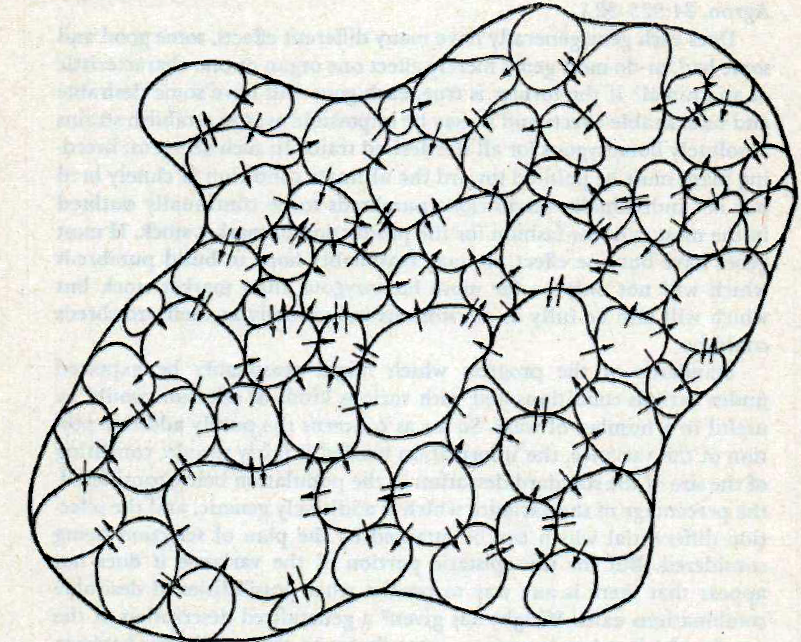
\includegraphics[width=\textwidth]{Figure_50.png}
    \caption{Subdivision of a breed into small local groups which exchange breeding
			 stock only at rare intervals and then only with neighboring local groups.}
    \label{fig:Lush_Figure_50}
\end{figure}

The consequence of such a separation into groups, each breeding
very largely within itself, would be that each such group would quickly
become more uniform than herds are today and that each group would
become different from other groups. Selection between the groups
would then be effective to an extent impossible today and unattainable
in the selection of individual animals for moderately or slightly heritable
characteristics, no matter how much the animal is studied nor how
skilled is the man who does the selection.

Many of these subgroups would begin to show undesired traits varying
in severity. Side by side with these, they would show other highly
desired traits more uniformly than present herds do. Groups showing
many desired and few undesired traits would be outcrossed mildly to
neighboring groups which were strong where they themselves were
weak. Then by renewed linebreeding with rigid selection for the traits
they wished to introduce by the outcross, the breeders would attempt to
fix the introduced desired traits without losing the desired traits they
already had. Groups showing few desired and many undesired traits
would either be discarded altogether or would be graded up by the continued
use of sires from the most successful groups until their individual
merit was restored or even exceeded that of the most successful group.
Then the breeders would start breeding within this group to find and
fix some one of the almost infinite number of desirable new combinations
of genes which would be possible. The general rule would be that
the more successful each subgroup was, the less readily would any outcrossing
be done and the milder such outcrossing would be.
\index{Breeding systems for varied purposes|)}

\section*{IMPORTANT PROBLEMS STILL UNSOLVED}
\index{Epistatic effects|(}

How generally important is epistasis? Do most gene substitutions
tend to produce the same effect when made in all kinds of individuals,
almost regardless of the other genes which are present? If so, inbreeding
systems are not so necessary for progress as has been implied here. But
the reverse may be true. It may be that nearly all genes, except lethals
and others which produce distinct breakdowns in the functioning of
vital organs, are epistatic in their effects. If so, inbreeding is even more
necessary for producing permanent changes than has been implied here,
and most of the progress which appears to be made by intensifying
selection is temporary and will disappear whenever the selection is relaxed.
There are only scraps of actual evidence about this in animals.
The results of Sprague and Tatum with corn indicate that most of the
hereditary differences in an unselected population are additive, but
that the differences which still remain between the survivors in an
intensely selected population are mostly epistatic. (Jour. Amer. Soc.
Agron. 34:923--32.)
\index{Epistatic effects|)}

Does each gene generally have many different effects\index{Multiple effects of genes}, some good and
some bad, or do most genes merely affect one organ or one characteristic
of an animal? If the former is true, each gene will have some desirable
and undesirable effects and it may be impossible ever to establish strains
absolutely homozygous for all the desired traits. In such an event, breeding
plans must be pointed toward the ultimate condition of closely bred
but not individually meritorious purebreds to be continually outbred
in the most extreme fashion for the production of market stock. If most
genes have but one effect, we may reasonably hope to build purebreds
which will not only be far more homozygous than market stock but
which will also be fully as meritorious individually as their crossbreds
could be.

Standards of the progress which might reasonably be expected
under various conditions and with various kinds of selection would be
useful in a number of ways. So far as concerns the purely additive portion
of the variance, the information needed is fairly simple, consisting
of the size of the standard deviation in the population being considered,
the percentage of the variance which is additively genetic, and the selection
differential which can be attained by the plan of selection being
considered. But for the epistatic portion of the variance it does not
appear that there is any way to predict what possibilities of desirable
combinations exist. Wright has given\footnote{\textit{Journal of Genetics},
30:243--66. Also \textit{Proc. Sixth International Cong. Genetics},
1:356-66.} a generalized description of the way in which epistatic variance
contributes to the correlation between relatives and of the general
consequences of selection where epistatic interactions are involved; but
it does not appear that this provides any way to predict when an epistatic
interaction of considerable importance may result from bringing together
genes which individually give no hint of the effects they will have when
combined. Probably that must remain a matter of trial and error.

Simple and reasonably complete objective ways of measuring the
practical merit of each animal would be very useful. For dairy cattle
and poultry there is an approach to that in weighing and testing the
milk and in counting and weighing the eggs, but other things also need
to be taken into account for these animals. For the other classes of animals
the standards for measuring practical merit are not even this well
developed. Considerably more needs to be done in developing practical
selection indexes which will pay attention to each practically important
characteristic without the risk of overemphasizing it.

Machinery for co-operating in animal breeding can doubtless be
made more efficient and useful. The dairy herd improvement associations
are an example of what can be done in this direction; but, if there
is to be any large increase in linebreeding in small herds or in community
breeding, closer co-operative organization aimed directly at that will
be essential. Bull circles may foreshadow the pattern which such efforts
will take.

\section*{OPPORTUNITIES IN ANIMAL BREEDING}
\index{Making new breeds|(}
\index{Opportunities in animal breeding|(}

The number of combinations of existing genes which have never yet
been brought together is practically infinite. In every breed there are
enough unfixed genes available to make possible the production of animals
more extreme than have ever yet existed in almost any direction
that the breeder might desire. All our breeds are still exceedingly plastic,
and the breeder's opportunities to mold them to his own desire are
so great that there is no occasion to mourn his inability to produce new
mutations at will and probably no important reason to regret that the
established breeding systems make it impossible for a breeder to use
blood from outside the breed unless he wishes to form a new breed of
his own. There is reason to think that a new breed could be formed
from crossing two or more of the existing breeds, but the plans and
specifications for doing that will probably require that the herd be at
least large enough to keep in service at all times three to five sires and a
much larger number of females. Otherwise, the inbreeding consequent
on the small number of animals which one man could manage would
be certain sooner or later to fix on the whole herd some undesired combinations
of parental traits . Also, in combining some of the extreme
characteristics of one breed with other extreme characteristics of another
breed it will be necessary to allow for several generations to permit
the desirable new combinations of genes to come together. How many
generations would be required to make a breed at least as uniform as
the breeds from which it was derived will, of course, depend upon how
many genes are involved in the differences between the breeds, how
many animals there are from which to select, how accurate the selections
are, how much linebreeding is done to those which appear to
come closest to the new combination desired and upon how homozygous
the parental breeds were. For example, if eight pairs of equally
important genes differ in the two parental breeds, the average breeding
value of the second crossbred generation (the $F_2$ generation) will differ
from the desired true-breeding combinations by four standard deviations.
It would be exceedingly unlikely that one could reach the goal in
as few as four more generations. If several different characteristics, each
dependent on several genes, are to be combined, it may well require
eight to ten generations of breeding after the original cross to come
reasonably close to the goal. This is not at all to say that making such a
breed is impossible but merely to call attention to the time which will
probably be required and to the need of budgeting that in the plans.
Partly offsetting this is the fact that the breeds which are to be used in
the cross are far from homozygous and that, by making more use of
inbreeding than is usually done, one might within two or three generations
from the first cross surpass the degree of homozygosity which
characterizes the parents.

Where the new ideal is an intermediate between the two breeds in
nearly all characteristics, rather than a mosaic of some characteristics
from one and other characteristics from the other, the first cross or second
cross generation may already average near the desired ideal. In that
case the generations required for selection to move the average to the
desired point would be unnecessary, and it would only remain to linebreed
intensively enough to increase homozygosity and uniformity to
the point that would warrant calling the new group a breed. These considerations
probably explain why most deliberate attempts to found a
breed have failed. The founders have not had large enough numbers to
carry on their own breeding plans without dangerously high inbreeding,
or else they have not had enough time to reach their goal before
they died. Not often were their heirs interested in continuing these
plans. Theoretically there seems to be no bar to forming a new breed in
this way if one has animals enough and time enough, but it is a rather
impressive fact that practically no breeds were formed thus. Extensive
mixing of races was involved in the founding of many breeds, but that
seems to have been undertaken for other reasons and was profitable as
it went along. Only incidentally and after some time had elapsed was
it observed that somewhere out of the welter of crossbreeding there
emerged a group which seemed to have merit enough that their owners
recognized them as a breed and sought to perpetuate them as such.

\index{Adaptation to local conditions!to tropics|(}
Currently the most active interest in forming new breeds is in tropical
and subtropical regions for which none of the established breeds
seem well suited. The Santa Gertrudis cattle in Texas; dairy cattle
suitable to Brazil, to the West Indies, and to India; and beef cattle for
the more tropical parts of South Africa, the Gold Coast and Kenya, arc
among the more striking examples. Generally the settlers in temperate
regions were able to find in Europe improved breeds which were
already fairly well suited to their needs. However, Corriedale sheep in
New Zealand, Columbia sheep in the United States, lard breeds of hogs
in the United States, Morgan, Standardbred, and American Saddle
Horses in the United States, all illustrate that even the temperate
regions have sometimes found it profitable to make their own breeds.
It is not likely that all of this which should be done has already been
accomplished, but it is clear that the difficulties in the way of forming a
new breed of farm animals are greater than in the way of forming a new
variety of plants. Recently formed breeds, such as the Hereford hog
and Palomino and Quarter horses, indicate that the process of breed
formation is not entirely ended but several breeds have been launched
and become popular and then have disappeared. Examples in the
United States are the Sapphire hog of about 1914 and the Mulefoot hog
of a decade earlier. Other examples of crossing which were aimed from
the very beginning at forming a new breed but did not succeed commercially
are the Bowlker herd of crosses between Guernseys and Holstein-
Friesians in the United States and the Tranekjaer herd of crosses
between Jerseys and Red Danish cattle in Denmark.
\noclub[3]
\index{Adaptation to local conditions!to tropics|)}
\index{Making new breeds|)}
\index{Opportunities in animal breeding|)}